
\documentclass[a4paper,11pt]{article}
\usepackage[utf8]{inputenc}
\usepackage[T1]{fontenc}
\usepackage[french]{babel}
\usepackage{graphicx}
\usepackage{hyperref}
\usepackage{geometry}
\usepackage{hyperref}
%\usepackage{enumitem}
%\geometry{margin=2.5cm}

\title{Documentation Utilisateur – Surveillance environnementale intelligente pour le campus}
\author{Marc Zaky, Iwen Nuss, Maxime Le Pelvé, Amaury Dubuc--Tabouy, Mathys Dubois}
\date{Année 2024-2025}

\begin{document}
	
	\maketitle
	
	\section*{Résumé}
	Ce document utilisateur vous guide dans l’utilisation du système de surveillance environnementale intelligente pour le campus. Il s’agit d’un dispositif de détection d’animaux basé sur un Raspberry Pi, avec une analyse automatisée des images à l’aide d’un traitement distribué via des fonctions serverless. Ce projet a été développé dans le cadre de l’étude pratique Mycélium.
	
	\tableofcontents
	\newpage
	
	\section{Notification Discord}
	La base de données est mise à jour toute les 24h. Lorsque celle-ci a bien été mise à jour sans problèmes techniques, vous recevrez une notification sur un serveur discord vous informant de l'actualisation des données de cette base de données, ainsi que quelques détails sur les données ajoutés.
	
	\subsection{Installation de Discord}
	Télécharger Discord via le site officiel : \url{https://discord.com/download}\\
	Puis cliquer sur "S'inscrire" afin de créer un compte.
	
	\subsection{Rejoindre le serveur}
	
	Cliquer ensuite sur ce lien afin de rejoindre le serveur  : \url{https://discord.gg/aRPNZEXe}\\
	Une fois sur ce serveur, vous pouvez voir deux salons: 
	\begin{itemize}
		\item Salon "Principal" : ce salon permet d'échanger librement entre les différents utilisateurs.
		\item Salon "Notif" : ce salon reçoit en temps réel les notifications du système sur la mise à jour de la base de donnée.
	\end{itemize}
	
	\subsection{Description des notifications}
	Les notifications envoyés par le système sont de la forme suivante : 
	\begin{figure}[ht]
		\centering
		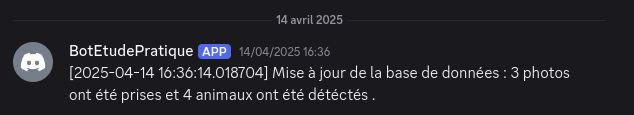
\includegraphics[scale=0.5]{Discord.png}
		\caption{Réception de la notification Discord}
		\label{fig5}
	\end{figure}
	
	Vous pouvez ainsi voir la date et l'heure à laquelle la notification a été reçu, le nombre de photos qui ont été prises ces 24h ainsi que le nombre total d'animaux qui ont été détectés parmi toutes ces photos.
	

	
	\section{Interface de visualisation des données}
	Cette interface permet de faire des requêtes sur la base de données afin de connaître et comprendre les données qui ont été capturés.
	
	\subsection{Connexion au serveur}
	Afin d'avoir accès à la base de données, il faut tout d'abord se connecter à distance au serveur qui héberge cette base.
	Pour cela, vous pouvez utiliser SSH qui permet de se connecter en ligne de commande à un autre ordinateur (serveur) de manière sécurisée, pour exécuter des commandes à distance.\\
	Taper \texttt{ssh utilisateur@adresse\_du\_serveur
	} \\
	A la suite de cette commande, il vous sera demandé votre clé SSH afin de compléter la connexion.
	
	\subsection{Ouverture de l'interface}
	Afin d'ouvrir l'interface, il vous suffit de taper la commande suivante dans le terminal en étant connecté au serveur : \texttt{python interface.py}\\
	Un nouvel onglet va s'ouvrir contenant l'interface.
	\begin{figure}[ht]
		\centering
		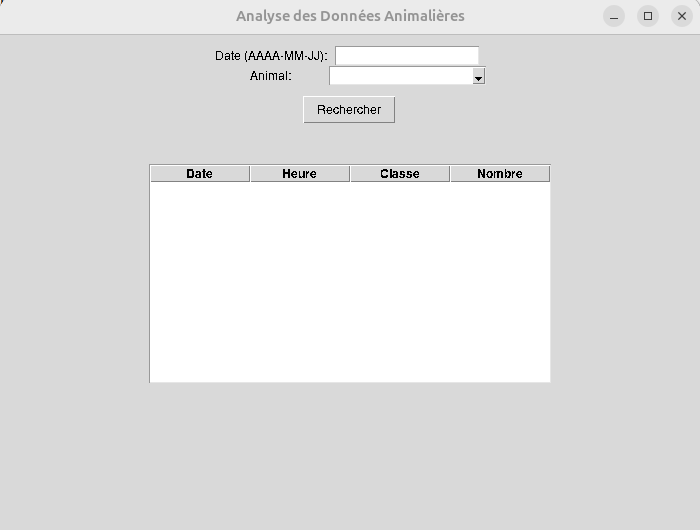
\includegraphics[scale=0.26]{interfaceVide.png}
		\caption{Ouverture de l'interface}
		\label{fig5}
	\end{figure}
	
	\subsection{Utilisation de l'interface}
	Afin d'afficher toutes les données présents dans la base de données, vous pouvez cliquer sur "Rechercher" sans ajouter de filtres.\\
	
	\begin{figure}[ht]
		\centering
		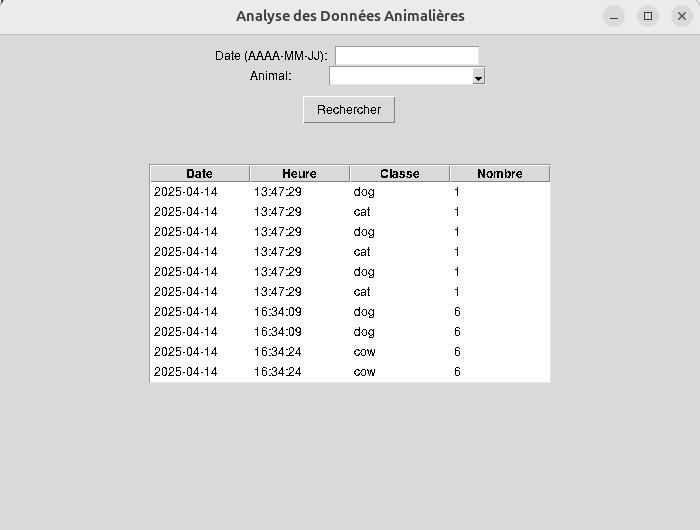
\includegraphics[scale=0.26]{interfacePleine.png}
		\caption{Données contenues dans la base}
		\label{fig5}
	\end{figure}
	
	Double cliquez sur une ligne afin d'afficher la photo correspondante.
	\begin{figure}[ht]
		\centering
		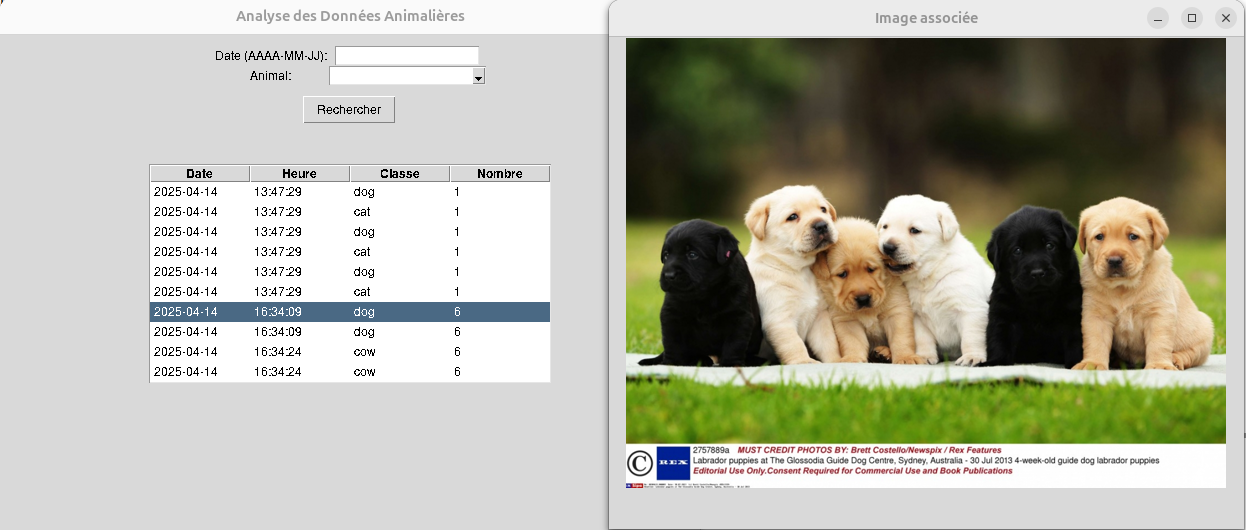
\includegraphics[scale=0.26]{interfaceImageAssocie.png}
		\caption{Image associée aux informations}
		\label{fig5}
	\end{figure}
	
	Vous pouvez aussi ajouter un filtre sur une date précise avec le format suivant : \texttt{AAAA-MM-JJ} et en cliquant sur "Rechercher"
	
	Un second filtre est disponible afin d'afficher uniquement toutes les photos d'un animal. Lorsque vous cliquez sur cette case, une liste déroulante contenant tous les animaux présents dans la base de donnée s'affiche.
	
	
	\section{Conclusion}
	Ce guide vous a présenté comment utiliser l’interface pour consulter les données issues de la surveillance environnementale, ainsi que la manière de recevoir des notifications via Discord. Grâce à ce système, vous pouvez facilement suivre l’activité animale sur le campus.
	
	\vspace{1em}
	
\end{document}
